\chapter{Conclusion and Future Work}
\label{conclusions}
\linenumbers

\paragraph{Discussion}
\label{par:7_discussion}
At this stage, we have completed our (partial) reverse engineering of the iTrust SWaT System, aiming to achieve a sufficient level of the physical process, or \textit{process comprehension}. 

\bigskip
Based on our analysis, we have identified a total of \textbf{49 properties} that are associated with the registers, their roles within the physical system, and their interactions with each other. These properties are summarized in Tables \ref{table:6_P1P2_summarize_properties}, \ref{table:6_P2P3_summarize_properties}, and \ref{table:6_P3P4_summarize_properties}. Additionally, we have reconstructed the \textbf{architecture of the four examined PLCs}, providing details on the registers they consist of and their respective characteristics. This architecture, along with the specific registers associated with each PLC, is presented in Table \ref{table:6_plc_registers_summary}.

Nonetheless, despite the limited availability of network traffic data, we have managed to derive a basic schematic of the PLC network and the communication pathways between them. Please note that this schematic may be incomplete due to the lack of comprehensive network traffic data. The reader can refer to Figure \ref{fig:6_network_SWaT} to visualize the network of PLCs.

The obtained \textit{process comprehension} enables us to plan a targeted attack on the system, utilizing the information we have gathered.

\bigskip
To evaluate the accuracy of the information obtained about the SWaT system, we can refer to Figure \ref{fig:7_swat_schema} \cite{swat_tecnical_pdf}, which provides a schematic representation of the SWaT system. An \texttt{x} indicates placement of sensors. By comparing the information derived from our analysis with the system schematic, we can assess the validity and reliability of our findings.

\begin{figure}[ht]
	\centering
	\includegraphics[scale=0.20]{chap7/swat_schema_1.png}
	\caption{iTrust SWaT schema}
	\label{fig:7_swat_schema}
\end{figure}

\bigskip
This image, while not comprehensive, serves to validate the accuracy of the properties derived from our system analysis of the first four stages of the SWaT system. It demonstrates that we have successfully identified the actuators and sensors within the system, and in some cases, we have even determined their specific roles within the physical process.

\bigskip
Figure \ref{fig:7_swat_hmi} \cite{swat_tecnical_pdf} provides an alternative representation of the SWaT system from the perspective of the Human-Machine Interface (HMI). This depiction complements the previous diagram by adding more contextual information and enhancing overall understanding of the system. It offers a comprehensive view of the system's components and their relationships, thereby improving the clarity and comprehension of the system's structure and functioning.

\begin{figure}[ht]
	\centering
	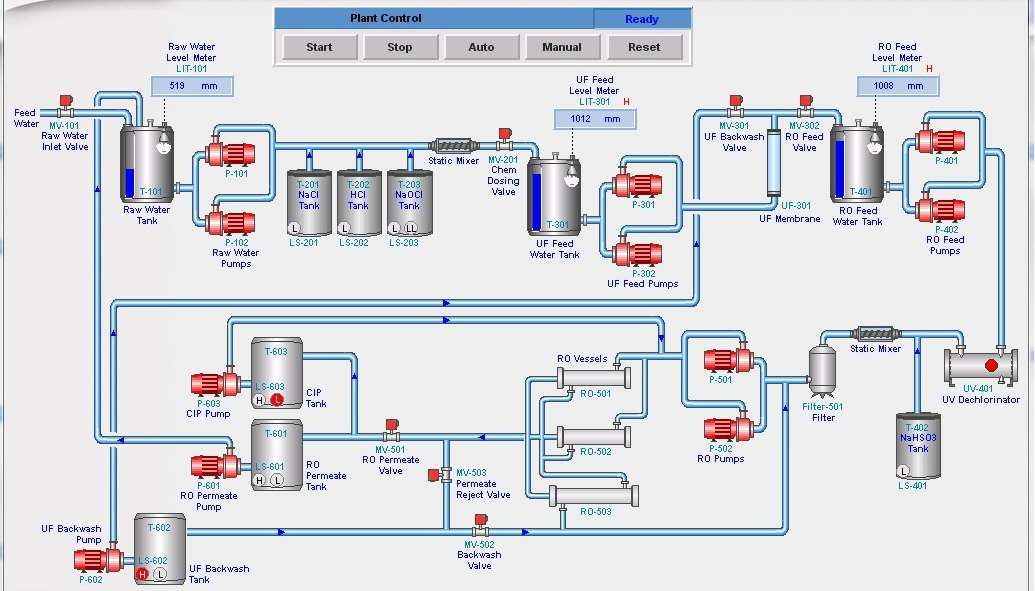
\includegraphics[scale=0.52]{chap7/hmi_swat.jpg}
	\caption{iTrust SWaT schema from HMI point of view.}
	\label{fig:7_swat_hmi}
\end{figure}

\bigskip
This figure introduces additional elements that were not included in the previous schematic shown in Figure \ref{fig:7_swat_schema}. It incorporates spare actuators and other components such as chemical tanks and the ultrafiltration membrane, which were not explicitly represented as registers in the available datasets. A comprehensive list of sensors and actuators, along with their respective functions within the system, can be found in the paper by Adepu et al. \cite{swat_dataset2015}.

%However, this figure also serves as further confirmation of the effectiveness of our analysis and the robustness of the framework we employed. Thus, we can confidently assert that \textbf{we have successfully achieved the objectives of this thesis}. We have not only validated the reverse engineering methodology introduced by Ceccato et al., but also improved and enhanced it through its practical application, making it more adaptable and valuable in real-world contexts.

\paragraph{Achievements of the approach}
\label{par:7_achievements}

After comparing the analysis results with the actual system, we can assess the extent to which the proposed framework has achieved its set objectives and identify any limitations encountered.

In terms of the objectives that have been achieved, either fully or partially, we have the following outcomes:

\begin{itemize}
	\item the proposed framework has effectively demonstrated independence from the specific system being examined;
	\item users have the ability to select a specific subsystem of their choice for analysis;
	\item automatic recognition of registers associated with physical process measurements and actuators (even spare actuators) has been implemented, including their actual operating ranges (\textit{relative setpoints});
	\item specific properties of actuators, including their states and the duration of each state, have been identified;
	\item recognition of which actuators handle incoming or outcoming flows;
	\item partial recognition of the roles of certain registers within the system has been achieved, such as tanks, valves, pumps, and flow/pressure sensors;
	\item conditions that cause state changes within the system (absolute setpoints) have been recognized;
	\item data perturbations for specific measurements have been attenuated;
	\item the Graphical Analysis component now provides a comprehensive view of the system under investigation, enabling the extraction of much more information compared to the corresponding functionality of the Ceccato et al. framework;
	\item the identification of invariants has been made easier, thanks in part to the implementation of semi-automated analyses;
	\item the process mining capabilities related to the physical system can extract more data compared to the Ceccato et al. framework;
	\item the reconstruction of the PLC network and the identification of the industrial protocol used for communications have been achieved.
\end{itemize}

\paragraph{Limitations of the approach} 
\label{par:7_limitations}
In terms of limitations, we have the following observations:

\begin{itemize}
	\item some specific register types or individual registers, such as valve \texttt{P3\_MV301}, sensor \texttt{P2\_AIT203}, or likely actuator \texttt{P4\_UV401}, could not have their roles identified;
	\item the presence and role of other system components, such as piping or filter membranes, could not be determined;
	\item due to highly incomplete and partial available network traffic data, it was not possible to integrate network traffic data into the Business Process Analysis phase;
	\item as a result of the aforementioned limitation, the Network Analysis phase is also incomplete, as it could not analyze communications occurring within the network via the CIP over EtherNet/IP protocol;
	\item both the integration of network traffic data and the comprehensive analysis of network communications are considered as future work, to be addressed when more consistent and complete data become available.
\end{itemize}

Based on our findings, we can confidently state that the proposed framework has successfully addressed many of the limitations identified in the Ceccato et al. framework. It has provided a greater amount of refined information, aligning with the goals set forth at the beginning of this thesis. However, it is important to acknowledge that certain limitations, particularly related to network data, have restricted the framework from fully realizing its potential. These limitations highlight the need for further advancements in gathering comprehensive and complete network data to unlock the framework's full capabilities.

\paragraph{Future work}
\label{par:7_futurework}
The framework, along with the thesis sources and analysis files, is openly accessible on the dedicated GitHub repository \cite{repository_tesi}. There is potential for further improvement and expansion of the framework. One possibility is integrating the analysis framework with an additional framework that utilizes the gathered data to generate targeted system attacks, building upon the writer's previous work as described in Section \ref{subsec:3_scan_preproc}.

Moreover, the proposed framework can benefit from various improvements and the introduction of specific new features to enhance its capabilities and effectiveness in analyzing industrial control systems. Here are some potential avenues for future work and enhancements to consider:

\begin{itemize}
	\item enhance the scanning and data gathering phase by reimplementing it to include support for multiple industrial protocols, in addition to Modbus. This improvement would enable the framework to detect and communicate with PLCs using various protocols commonly used in ICS environments, expanding its compatibility and usability;
	
	\item enhance the automatic recognition of sensors and actuators by leveraging advanced machine learning and artificial intelligence techniques. This improvement would involve training models to accurately identify and classify different types of sensors and actuators based on their data patterns and characteristics;
	
	\item complete the implementation of network traffic data within the Business Process part of the framework. However, it is crucial to ensure that the network traffic data and physical process data used for analysis are reliable and not compromised by external attackers, as accurate and untampered data is essential for effective analysis;
	
	\item implement an automated system for recognizing real system configurations by excluding actuators that do not significantly contribute to changing the system behavior within the analyzed PLC. This automatic recognition system can save time and effort by eliminating the need to manually filter out non-contributing actuators during the analysis process.
\end{itemize}

\vfill
\nolinenumbers